\subsection{Indymo}
Indymo uses aquatic drones to collect underwater images, water samples and water quality and ecology data for public and private entities who want to inspect and monitor water systems. These drones are equipped with water quality sensors to collect data. Indymo has deployed their underwater drones in several countries such as the Netherlands, Vietnam, and Indonesia. \cite{indymoindonesia}

The primary purpose of these drones is to perform water quality mapping and monitoring of floating structures

As seen in an article published April 2020 \cite{indymoarticle}, Indymo tested multiple underwater drones (ROVs), each of them having with different characteristics. ROVs seem to have a generally a large payload capability which allows for bulky multi-parameter probes to be mounted on the ROV, probes normally used by hand.

\begin{figure}[h]
\centering
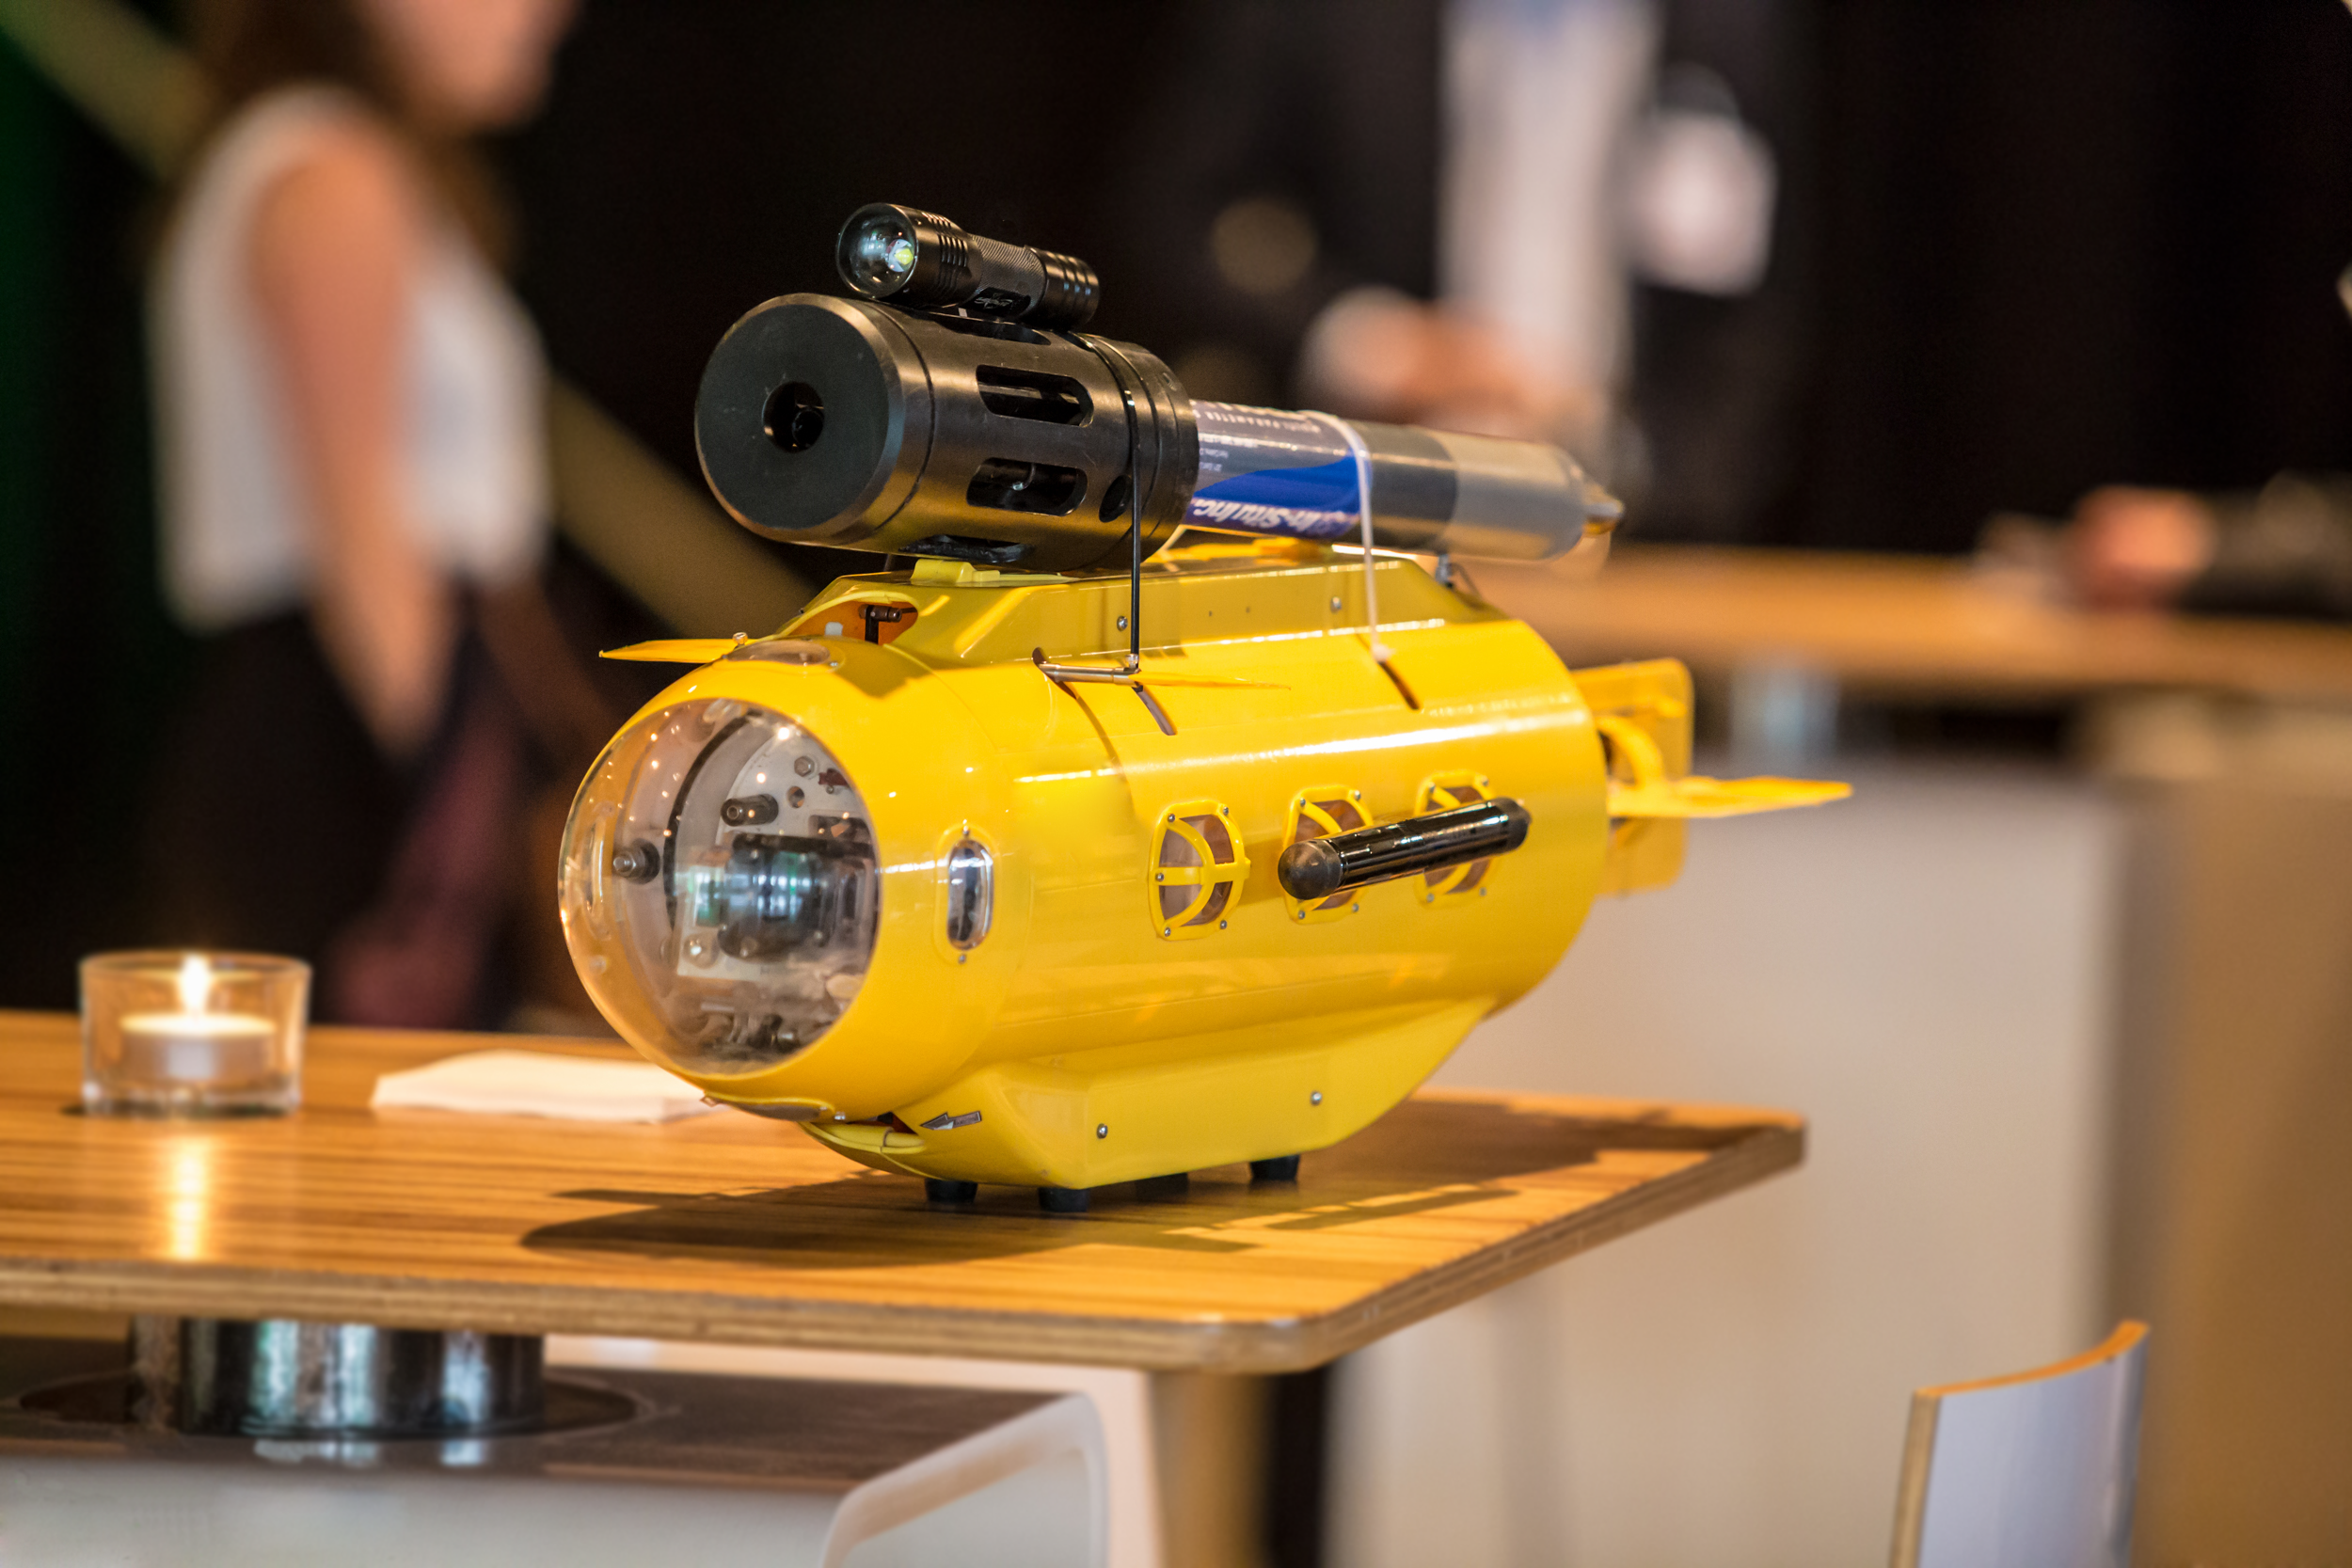
\includegraphics[scale=0.5]{similarprojects/11_innodrone.jpg}
\caption{Indymo's Innodrone (Based on the Thunder Tiger Neptune) \cite{indymoarticle}}
\end{figure}

They seem to measure water quality variables like pressure, temperature, conductivity, dissolved oxygen, algae and turbidity using one to two probes. Data was collected every 10s, and seem to be saved on the probes itself. Operational staff collected data simultaneously using conventional methods to validate the sensor data.

Indymo listed several multi-parameter probes they used throughout their research. They were very much of use as they gave insight as to what standards there are regarding water quality measurement precision.

\subsubsection{Similarity}
Indymo uses underwater ROVs for a 3D scan of the water, while this project focuses on using aerial UAVs to get a surface scan of the water. Both ways have its benefits and drawbacks, with Indymo's devices getting much more detailed information at the cost of man power and lack of automation.

